\chapter{Sintesis Total: Strategi dan Rute Klasik}\label{ch:b3:total-synthesis}

Obat antikanker paklitaksel pertama kali diisolasi dari kulit kayu pohon yew
Pasifik, pohon yang tumbuh lambat; pengupasan kulit kayu itu mematikan pohonnya, dan pasokannya
jauh di bawah kebutuhan pasien. Para kimiawan menjawabnya dengan dua cara: \omterm{def:b3:total-synthesis:total}{sintesis
total}, yang membuktikan bahwa molekul itu dapat dibangun dari bahan awal yang
sederhana tetapi terlalu panjang untuk produksi, dan \omterm{def:b3:total-synthesis:total}{semisintesis} dari senyawa
kerabat yang diekstraksi dari daun jarum pohon yew biasa, yang dapat diperbarui.
Bab ini membahas bagaimana rute-rute semacam itu dinilai dan dirancang: bagaimana rendemen
saling mengalikan, mengapa konvergensi menguntungkan, berapa biaya gugus pelindung, ikatan mana yang
dibuat lebih dahulu, dan tiga sintesis tonggak yang dibaca dengan perangkat itu.

\begin{recall}
Jilid Tahun 2 membahas analisis retrosintesis (molekul target,
diskoneksi, sinton, ekuivalen sintetis, interkonversi gugus
fungsi), gugus pelindung ortogonal, reaksi aldol,
anulasi Robinson, reaksi Wittig, dan kimia iminium; Jilid Tahun 1
membahas gugus pelindung dan rendemen. \Cref{ch:b3:asymmetric-synthesis},
\cref{ch:b3:pericyclic}, dan \cref{ch:b3:homogeneous-catalysis} menyediakan
tahap-tahap kunci modern.
\end{recall}

\begin{omfigure}
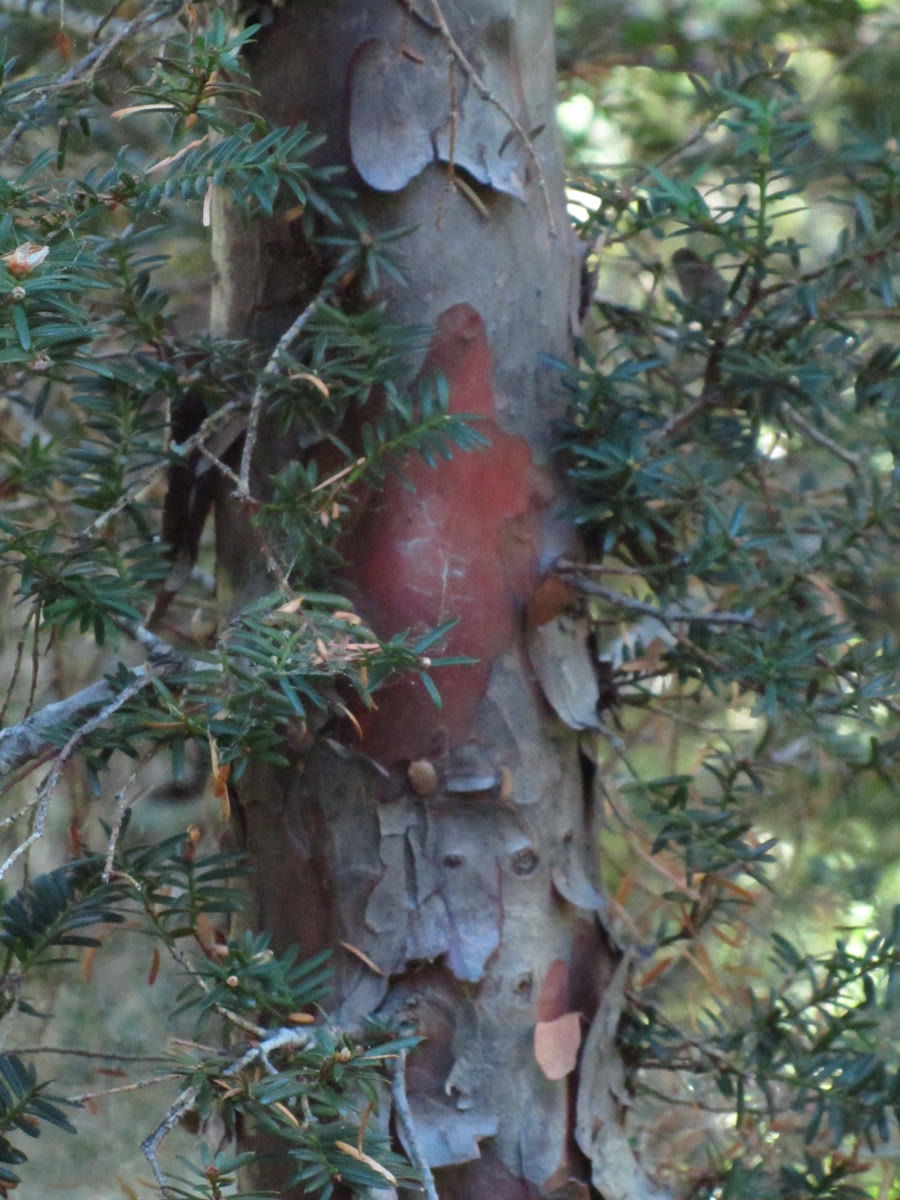
\includegraphics[width=0.32\linewidth]{images/book4/pacific-yew.jpg}

{\small Kulit kayu dan daun jarum pohon yew Pasifik, sumber pertama paklitaksel.
Foto: JOE BLOWE, CC BY-SA 2.0.}
\end{omfigure}

\section{Mengukur sebuah sintesis}

\begin{definition}[Sintesis total]\label{def:b3:total-synthesis:total}
Yang disebut \emph{sintesis total}\index{sintesis total} adalah sintesis yang membuat molekul kompleks, sering
sebuah produk alam, dari senyawa komersial yang sederhana. Yang disebut \emph{sintesis
formal}\index{sintesis formal} adalah sintesis yang membuat sebuah zat antara dari sintesis total
terdahulu, sehingga melengkapi rute itu di atas kertas. Yang disebut \emph{semisintesis}\index{semisintesis}
adalah sintesis yang dimulai dari senyawa alam yang sudah dekat dengan target.
\end{definition}

\begin{definition}[Arsitektur rute]\label{def:b3:total-synthesis:architecture}
Dalam \emph{sintesis linear}\index{sintesis linear}, setiap tahap bekerja pada
produk tahap sebelumnya; dalam \emph{sintesis konvergen}\index{sintesis konvergen},
fragmen-fragmen yang terpisah dibuat secara paralel dan digabungkan pada akhir. Yang disebut
\emph{urutan linear terpanjang}\index{urutan linear terpanjang} (LLS) adalah
jumlah tahap terbesar dari bahan awal mana pun sampai target. Yang disebut
\emph{rendemen keseluruhan}\index{rendemen keseluruhan} adalah jumlah target yang diperoleh
dibagi dengan jumlah bahan awal pembatas.
\end{definition}

\begin{proposition}[Rendemen keseluruhan]\label{prop:b3:total-synthesis:overall-yield}
Untuk serangkaian tahap dengan rendemen $y_1, \dots, y_n$, \omterm{def:b3:total-synthesis:architecture}{rendemen keseluruhannya} adalah $Y = \prod_i y_i$.
\end{proposition}

\begin{proof}
Setiap tahap mengubah jumlah yang diterimanya menjadi produk sebanyak $y_i$ kali jumlah itu; jumlah
yang mencapai target adalah jumlah awal yang dikalikan dengan setiap faktor secara
berurutan.
\end{proof}

\begin{proposition}[Konvergensi]\label{prop:b3:total-synthesis:convergent}
Rute dengan $n = 2m + 1$ tahap yang rendemennya sama $y$, yang dibangun sebagai dua cabang dengan $m$ tahap yang digabungkan oleh
satu tahap kopling, memiliki \omterm{def:b3:total-synthesis:architecture}{rendemen keseluruhan} $y^{m+1}$ sepanjang \omterm{def:b3:total-synthesis:architecture}{urutan linear terpanjangnya},
dibandingkan dengan $y^{2m+1}$ untuk rute linear dengan tahap-tahap yang sama.
\end{proposition}

\begin{proof}
Setiap cabang dibuat secara terpisah, dari bahan awal sebanyak yang diperlukan:
bahan setiap cabang melewati $m$ tahap lalu kopling, yaitu $m + 1$
faktor $y$. Dalam rute linear, bahan itu melewati semua $2m + 1$ tahap. Untuk $m = 10$
dan $y = 0.90$: 31\,\% dibandingkan dengan 11\,\%.
\end{proof}

\begin{omfigure}
\begin{tikzpicture}
\begin{axis}[width=0.7\linewidth, height=5.8cm, xmin=0, xmax=30, ymin=0, ymax=1.02,
  axis lines=left, xlabel={jumlah tahap $n$}, ylabel={rendemen keseluruhan},
  tick label style={font=\scriptsize}, label style={font=\small},
  legend style={font=\scriptsize, draw=none, at={(1.03,0.5)}, anchor=west}, legend cell align=left]
\addplot[color=omDef, thick] table[x=n, y=y95] {figdata/out/bachelor-3-overall-yield.dat};
\addlegendentry{95\,\% per tahap}
\addplot[color=omMeth, thick] table[x=n, y=y90] {figdata/out/bachelor-3-overall-yield.dat};
\addlegendentry{90\,\%}
\addplot[color=omThm, thick] table[x=n, y=y80] {figdata/out/bachelor-3-overall-yield.dat};
\addlegendentry{80\,\%}
\addplot[color=omMeth, thick, dashed, mark=*, mark size=1pt] table[x=n, y=y90] {figdata/out/bachelor-3-overall-yield-b.dat};
\addlegendentry{90\,\%, konvergen}
\end{axis}
\end{tikzpicture}

{\small \omterm{def:b3:total-synthesis:architecture}{Rendemen keseluruhan} terhadap jumlah tahap untuk tiga rendemen per tahap
(garis utuh: rute linear), dan untuk rute konvergen pada 90\,\% per tahap (dua
cabang yang sama digabungkan pada tahap terakhir; putus-putus). Dua puluh tahap pada 90\,\% menyisakan 12\,\%; tahap-tahap
yang sama yang disusun secara konvergen menyisakan sekitar tiga kali lebih banyak.}
\end{omfigure}

\begin{omfigure}
\begin{tikzpicture}[font=\scriptsize, >=Stealth, node distance=0.9cm,
  st/.style={circle, draw, fill=omDef!15, minimum size=4mm, inner sep=0pt}]
  \foreach \i in {0,...,6} { \node[st] (l\i) at (\i*0.9,1.6) {}; }
  \foreach \i in {0,...,5} { \pgfmathtruncatemacro\j{\i+1} \draw[->] (l\i) -- (l\j); }
  \node[anchor=west] at (6.0,1.6) {linear: 6 tahap, LLS 6};
  \foreach \i in {0,...,2} { \node[st] (a\i) at (\i*0.9,0.6) {}; \node[st] (b\i) at (\i*0.9,-0.6) {}; }
  \draw[->] (a0) -- (a1); \draw[->] (a1) -- (a2); \draw[->] (b0) -- (b1); \draw[->] (b1) -- (b2);
  \node[st, fill=omThm!25] (t) at (3.0,0) {};
  \draw[->] (a2) -- (t); \draw[->] (b2) -- (t);
  \node[anchor=west] at (3.4,0) {konvergen: 5 tahap, LLS 3};
\end{tikzpicture}

{\small Pohon rute: setiap lingkaran adalah sebuah senyawa, setiap panah sebuah tahap. Rute linear
melewatkan seluruh bahannya melalui setiap tahap; rute konvergen membuat dua fragmen
berdampingan lalu mengoplingnya, sehingga \omterm{def:b3:total-synthesis:architecture}{urutan linear terpanjangnya} lebih pendek.}
\end{omfigure}

\begin{definition}[Ekonomi dan idealitas]\label{def:b3:total-synthesis:economy}
Yang disebut \emph{ekonomi tahap}\index{ekonomi tahap} adalah tujuan untuk mencapai target dengan
tahap sesedikit mungkin; \emph{ekonomi gugus pelindung}\index{ekonomi gugus pelindung}
adalah tujuan untuk memakai tahap proteksi dan deproteksi sesedikit mungkin. Yang disebut
\emph{idealitas}\index{idealitas} sebuah rute adalah fraksi tahapnya yang
membangun kerangka atau membuat perubahan tingkat oksidasi yang diperlukan:
$(\text{tahap konstruksi} + \text{tahap redoks strategis})/(\text{total tahap})$.
\end{definition}

\begin{proposition}[Idealitas sebuah rute]\label{prop:b3:total-synthesis:ideality}
Rute satu wadah yang hanya membentuk ikatan-ikatan kerangka memiliki \omterm{def:b3:total-synthesis:economy}{idealitas} 100\,\%; setiap tahap proteksi,
deproteksi, interkonversi gugus fungsi, atau redoks nonstrategis
menurunkannya.
\end{proposition}

\begin{proof}
Langsung dari definisinya: tahap-tahap semacam itu menambah penyebut tanpa menambah
pembilang.
\end{proof}

\section{Gugus pelindung dan ekonominya}

Setiap gugus pelindung memerlukan paling sedikit dua tahap, pereaksi untuk memasang dan
melepaskannya, serta bahan yang hilang pada keduanya. Rute delapan tahap pada 90\,\% menyisakan
43\,\% bahannya; menambahkan dua proteksi dan dua deproteksi masing-masing pada 95\,\%
menurunkannya menjadi 35\,\%. Gugus pelindung dipilih ortogonal, sehingga masing-masing dapat
dilepaskan tanpa menyentuh yang lain; lebih baik lagi, urutan tahap-tahap
diatur sedemikian rupa sehingga gugus reaktif itu belum ada, atau belum dimunculkan, ketika
gugus itu akan mengganggu: sintesis tanpa gugus pelindung adalah sebuah tujuan, bukan sekadar keanehan.

\begin{method}[Membaca sebuah sintesis total]\label{met:b3:total-synthesis:analyse}
\begin{enumerate}
  \item Kenali cincin, pusat stereo, dan gugus-gugus sensitif target.
  \item Carilah diskoneksi-diskoneksi kunci dan reaksi-reaksi yang membuatnya ke arah
        maju (\omterm{def:b3:total-synthesis:strategic-bond}{ikatan strategis}).
  \item Hitunglah tahap-tahapnya dan carilah \omterm{def:b3:total-synthesis:architecture}{urutan linear terpanjang}; catatlah konvergensinya.
  \item Catatlah bagaimana setiap pusat stereo ditetapkan (kendali substrat, auksiliari, katalis,
        \omterm{def:b3:asymmetric-synthesis:chiral-pool}{kumpulan kiral}).
  \item Daftarlah gugus pelindung dan tahap-tahap tidak ideal lainnya; hitunglah \omterm{def:b3:total-synthesis:architecture}{rendemen
        keseluruhan} dan \omterm{def:b3:total-synthesis:economy}{idealitasnya}.
\end{enumerate}
\end{method}

\begin{method}[Menghitung tahap]\label{met:b3:total-synthesis:count}
\begin{enumerate}
  \item Sebuah tahap adalah satu operasi yang berakhir dengan produk yang diisolasi (atau setidaknya sudah dikerjakan);
        urutan satu wadah tanpa isolasi dihitung sebagai satu tahap.
  \item Hitunglah semua tahap untuk jumlah totalnya; untuk LLS, ikutilah jalur terpanjang dari
        senyawa komersial sampai target.
  \item Kalikan rendemen-rendemen sepanjang LLS untuk memperoleh \omterm{def:b3:total-synthesis:architecture}{rendemen keseluruhan}.
\end{enumerate}
\end{method}

\section{Ikatan strategis dan tahap-tahap kunci pembentuk cincin}

\begin{definition}[Ikatan strategis]\label{def:b3:total-synthesis:strategic-bond}
Yang disebut \emph{ikatan strategis} sebuah target\index{ikatan strategis} adalah ikatan yang
diskoneksinya paling menyederhanakan target, biasanya dengan memecah sistem cincin
atau menghilangkan beberapa pusat stereo sekaligus, dan yang dapat dibentuk oleh reaksi yang
andal.
\end{definition}

Reaksi pembentuk cincin yang membuat dua ikatan atau beberapa pusat stereo sekaligus
adalah andalannya: reaksi Diels--Alder (dua ikatan C--C, sampai empat
pusat stereo, secara stereospesifik, \cref{ch:b3:pericyclic}), anulasi
Robinson (cincin beranggota enam pada sebuah keton), \omterm{def:b3:homogeneous-catalysis:metathesis}{metatesis penutupan cincin}
(\cref{ch:b3:homogeneous-catalysis}) untuk cincin sedang dan besar, serta kaskade.

\begin{definition}[Reaksi kaskade]\label{def:b3:total-synthesis:cascade}
Yang disebut \emph{reaksi kaskade}\index{reaksi kaskade} adalah serangkaian
transformasi yang setiap tahapnya menciptakan gugus fungsi untuk tahap berikutnya,
tanpa mengisolasi zat antara atau menambahkan pereaksi.
\end{definition}

\begin{definition}[Sintesis biomimetik]\label{def:b3:total-synthesis:biomimetic}
Yang disebut \emph{sintesis biomimetik}\index{sintesis biomimetik} adalah sintesis yang meniru rute
yang diduga dipakai organisme untuk membuat sebuah produk alam.
\end{definition}

Siklisasi skualena oksida menjadi lanosterol di dalam sel, yaitu empat cincin dan tujuh
pusat stereo dalam satu kaskade enzimatis, mengilhami siklisasi poliena
William Johnson, tempat sebuah kation yang dimulai di satu ujung poliena yang dirancang dengan cermat
menutup cincin demi cincin melalui keadaan-keadaan transisi mirip kursi, sehingga menetapkan
fusi cincin \textit{trans} pada steroid.

\section{Rute-rute tonggak}

\begin{definition}[Reaksi Mannich]\label{def:b3:total-synthesis:mannich}
Yang disebut \emph{reaksi Mannich}\index{reaksi Mannich} adalah adisi enol
atau enolat pada ion iminium, yang dibuat langsung di dalam campuran reaksi dari aldehida dan amina primer atau
sekunder, sehingga terbentuk senyawa $\beta$-amino karbonil.
\end{definition}

Pada 1917 Robert Robinson membuat tropinon, inti bisiklik atropina dan
kokaina, dalam satu wadah dari tiga komponen sederhana dalam air, sambil membayangkan bahwa
tumbuhan mungkin membangunnya dengan cara yang sama:
$\ce{C4H6O2 + CH3NH2 + C5H6O5 -> C8H13NO + 2CO2 + 2H2O}$ (suksinaldehida, metilamina, dan
asam asetondikarboksilat memberikan tropinon).

\begin{omfigure}
\begin{tikzpicture}[font=\small, >=Stealth]
  \node[align=center] at (-0.5,0) {$\ce{OHC-CH2CH2-CHO}$\\ $+\ \ce{CH3NH2}$\\ $+\ \ce{HO2C-CH2-CO-CH2-CO2H}$};
  \draw[->, thick] (3.0,0) -- (4.7,0) node[midway, above, font=\scriptsize] {air berbufer} node[midway, below, font=\scriptsize] {$-\ce{2CO2}$, $-\ce{2H2O}$};
  \begin{scope}[xshift=6.1cm, yshift=-0.2cm]
    \coordinate (c1) at (-1,0.3); \coordinate (c2) at (-0.8,-0.5); \coordinate (c3) at (0,-0.9);
    \coordinate (c4) at (0.8,-0.5); \coordinate (c5) at (1,0.3); \coordinate (c6) at (0.45,1.15);
    \coordinate (c7) at (-0.45,1.15); \coordinate (n) at (0,0.45);
    \draw[thick] (c1) -- (c2) -- (c3) -- (c4) -- (c5) -- (c6);
    \draw[thick] (c7) -- (c1);
    \draw[thick] (c6) -- (0.12,1.15); \draw[thick] (-0.12,1.15) -- (c7);
    \draw[thick] (c1) -- (n) -- (c5);
    \draw[thick] (n) -- (0,1.6) node[above, inner sep=1pt] {$\ce{CH3}$};
    \draw[thick, double, double distance=1.5pt] (c3) -- (0,-1.55) node[below, inner sep=1pt] {O};
    \node[fill=white, inner sep=0.5pt] at (n) {N};
    \node[font=\scriptsize, anchor=west] at (1.2,0.3) {tropinon};
  \end{scope}
\end{tikzpicture}

{\small Sintesis tropinon Robinson. Dua \omterm{def:b3:total-synthesis:mannich}{reaksi Mannich}, yang pertama
antarmolekul dan yang kedua menutup cincin, menggabungkan ketiga komponen;
kedua gugus asam karboksilat yang membuat gugus-gugus $\ce{CH2}$ tengah dapat mengenol lalu
lepas sebagai karbon dioksida. Dalam produk bisiklik itu, jembatan N-metil merentangi
cincin beranggota tujuh.}
\end{omfigure}

\begin{proposition}[Tropinon dalam satu wadah]\label{prop:b3:total-synthesis:tropinone}
Sintesis tropinon satu wadah terdiri atas dua \omterm{def:b3:total-synthesis:mannich}{reaksi Mannich} yang diikuti oleh dua
dekarboksilasi.
\end{proposition}

\begin{proof}[Argumen]
Metilamina dan satu gugus aldehida suksinaldehida memberikan ion iminium; sebuah
enol asam asetondikarboksilat teradisi padanya (Mannich pertama). Amina sekunder
yang terbentuk berkondensasi dengan gugus aldehida kedua menjadi ion iminium siklik,
yang diserang oleh enol di sisi lain keton (Mannich kedua),
sehingga bisiklus itu tertutup. Kedua gugus asam $\beta$-keto lalu melepaskan $\ce{CO2}$, seperti yang dialami asam $\beta$-keto
pada pemanasan ringan.
\end{proof}

Sintesis prostaglandin $\mathrm F_{2\alpha}$ oleh Elias Corey (1969) membuat analisis retrosintesis
menjadi eksplisit. Sebuah bisiklo[2.2.1]heptenon yang dibangun dengan reaksi Diels--Alder membawa
konfigurasi relatif substituen-substituen siklopentana; \omterm{def:b3:radicals-carbenes:baeyer}{oksidasi
Baeyer--Villiger} (\cref{ch:b3:radicals-carbenes}) dan
iodolaktonisasi mengubahnya menjadi lakton Corey, yang menjadi tempat kedua rantai samping
dipasang melalui olefinasi. Lakton itu telah dipakai untuk banyak obat prostaglandin
sejak saat itu.

\begin{omfigure}
\begin{tikzpicture}[font=\small,
  box/.style={draw, rounded corners, align=center, fill=omDef!8, inner sep=4pt}]
  \node[box] (t) at (0,0) {prostaglandin\\ $\mathrm F_{2\alpha}$};
  \node[box] (l) at (4.4,0) {lakton Corey\\ (empat\\ pusat stereo)};
  \node[box] (b) at (9.2,0) {bisiklo[2.2.1]-\\ heptenon};
  \node[box] (d) at (9.2,-2.4) {siklopentadiena\\ tersubstitusi $+$\\ ekuivalen keten};
  \draw[omretro] (t) -- (l) node[midway, above=3pt, font=\scriptsize] {olefinasi};
  \draw[omretro] (l) -- (b) node[midway, above=3pt, font=\scriptsize, align=center] {iodolaktonisasi,\\ Baeyer--Villiger};
  \draw[omretro] (b) -- (d) node[midway, right, font=\scriptsize] {Diels--Alder};
\end{tikzpicture}

{\small Retrosintesis prostaglandin $\mathrm F_{2\alpha}$ oleh Corey, secara garis besar (panah ganda: ``dibuat
dari''). Kedua rantai samping didiskoneksi lebih dahulu; siklopentana beserta
keempat pusat stereonya berasal dari sebuah lakton, lakton itu dari keton bisiklik,
dan keton itu dari reaksi Diels--Alder yang menetapkan konfigurasi relatifnya.}
\end{omfigure}

Oseltamivir, obat influenza, dibuat secara industri dari asam sikimat, senyawa
\omterm{def:b3:asymmetric-synthesis:chiral-pool}{kumpulan kiral} yang diekstraksi dari bunga lawang dan kemudian diproduksi melalui
fermentasi: cincin beranggota enamnya dan pusat-pusat stereonya sudah tersedia di tempatnya.
Rute itu mengubah diol cincin menjadi epoksida, membukanya dengan azida, menutup
sebuah aziridina dan membukanya lagi dengan azida, sehingga kedua atom nitrogen ditetapkan
\textit{trans}; asetilasi dan reduksi menyelesaikan pekerjaannya. Karena natrium azida dan
azida organik beracun dan berpotensi meledak pada skala besar, rute-rute bebas azida
kemudian dikembangkan.

\begin{omfigure}
\begin{tikzpicture}[font=\scriptsize, >=Stealth,
  box/.style={draw, rounded corners, align=center, fill=omMeth!8, inner sep=3pt}]
  \node[box] (a) at (0,0) {asam ($-$)-sikimat\\ (kumpulan kiral)};
  \node[box] (b) at (3.1,0) {ester, ketal,\\ mesilat};
  \node[box] (c) at (6.0,0) {epoksida};
  \node[box] (d) at (8.6,0) {azido alkohol};
  \node[box] (e) at (8.6,-1.5) {aziridina};
  \node[box] (f) at (5.4,-1.5) {prekursor diamina\\ \textit{trans} (azida)};
  \node[box] (g) at (1.6,-1.5) {oseltamivir\\ fosfat};
  \draw[->] (a) -- (b); \draw[->] (b) -- (c); \draw[->] (c) -- (d) node[midway, above] {$\ce{N3-}$};
  \draw[->] (d) -- (e); \draw[->] (e) -- (f) node[midway, above] {$\ce{N3-}$};
  \draw[->] (f) -- (g) node[midway, below, align=center] {asetilasi,\\ reduksi};
\end{tikzpicture}

{\small Oseltamivir dari asam sikimat, hanya tahap-tahap kuncinya: cincin alami beserta
pusat-pusat stereonya dipertahankan, dan dua atom nitrogen dimasukkan secara \textit{trans} satu terhadap yang lain
melalui pembukaan berturut-turut sebuah epoksida dan sebuah aziridina dengan azida.}
\end{omfigure}

\section{Dari penemuan ke proses}

Rute yang menghasilkan miligram untuk uji biologis jarang merupakan rute yang dipakai
untuk berton-ton. Para kimiawan proses menelusuri rute-rute berdasarkan biaya, keamanan, dan ketangguhan:
mereka menghilangkan kromatografi dan menggantinya dengan kristalisasi, mengganti pereaksi
berbahaya dan suhu kriogenik, memperpendek urutan, memeriksa keamanan termal
setiap tahap dengan kalorimetri, dan menetapkan spesifikasi untuk pengotor.
Pilihan-pilihan ini bertemu dengan ukuran-ukuran pada \cref{ch:b3:green-industrial}.

\begin{inthelab}[Dari satu gram ke satu kilogram]
Sebuah tahap yang dijalankan pada satu gram dalam labu alas bulat diulang pada sepuluh gram dalam
reaktor berselubung dengan pengaduk atas dan probe suhu di dalam
cairan, dengan menambahkan pereaksi yang reaktif pada laju terkendali sambil memantau
suhu internal: kalor yang dilepaskan tumbuh bersama volume, tetapi luas yang
menyingkirkannya hanya tumbuh sebagai kuadrat ukuran. Hanya jika aliran kalor dan pengerjaannya
(pemisahan fase, penyaringan, pengeringan) berperilaku baik, tahap itu dijalankan pada skala satu kilogram.
\end{inthelab}

\begin{safety}{\ghs[0.62cm]{GHS06}\ghs[0.62cm]{GHS08}\ghs[0.62cm]{GHS09}}
% ledger: ghs4:NaN3
Natrium azida: fatal jika tertelan, sangat beracun bagi kehidupan akuatik; dengan asam, zat itu
melepaskan asam hidrazoat, gas yang beracun dan eksplosif, dan dengan logam berat
(tembaga dan timbal di saluran pembuangan) membentuk azida yang eksplosif. Limbahnya dimusnahkan
secara kimia, tidak pernah dibuang begitu saja.
\end{safety}

\begin{history}[Robinson, Woodward, Corey]
Robert Robinson menerima Hadiah Nobel Kimia 1947 untuk karyanya tentang
alkaloid dan produk tumbuhan lainnya; sintesis tropinonnya pada 1917 masih
dikutip karena keekonomisannya. Sintesis-sintesis Robert Woodward untuk kinina, kolesterol,
klorofil, dan, bersama Albert Eschenmoser, vitamin $\mathrm B_{12}$ menjadikan \omterm{def:b3:total-synthesis:total}{sintesis total} sebuah seni
(hadiah 1965). Elias Corey memformalkan analisis retrosintesis dan menerima
hadiah 1990 untuk teori dan metodologi sintesis organik.
\end{history}

\section{Latihan}

\begin{exercise}[$\star$]\label{exo:b3:total-synthesis:1}
Hitunglah \omterm{def:b3:total-synthesis:architecture}{rendemen keseluruhan} rute linear 10 tahap dan 20 tahap pada 90\,\% dan pada 80\,\% per
tahap.
\end{exercise}

\begin{exercise}[$\star$]\label{exo:b3:total-synthesis:2}
Sebuah rute membuat fragmen A dalam lima tahap dan fragmen B dalam tiga tahap, mengopling keduanya, dan
memerlukan empat tahap lagi sampai target. Berikan jumlah total tahap dan
\omterm{def:b3:total-synthesis:architecture}{urutan linear terpanjangnya}.
\end{exercise}

\begin{exercise}[$\star$]\label{exo:b3:total-synthesis:3}
Berikan produk \omterm{def:b3:total-synthesis:mannich}{reaksi Mannich} aseton, formaldehida, dan
dimetilamina.
\end{exercise}

\begin{exercise}[$\star$]\label{exo:b3:total-synthesis:4}
Berikan diskoneksi Diels--Alder untuk 4-asetilsikloheksena, serta reaksi
majunya.
\end{exercise}

\begin{exercise}[$\star\star$]\label{exo:b3:total-synthesis:5}
Sebuah rute linear 21 tahap berjalan pada 90\,\% per tahap. Hitunglah \omterm{def:b3:total-synthesis:architecture}{rendemen keseluruhannya} dan rendemen
versi konvergennya dengan dua cabang 10 tahap dan satu kopling.
\end{exercise}

\begin{exercise}[$\star\star$]\label{exo:b3:total-synthesis:6}
Rute A memiliki 12 tahap, 7 di antaranya membuat ikatan kerangka dan 1 merupakan reduksi
strategis; rute B memiliki 9 tahap, 7 di antaranya bersifat kerangka. Hitunglah \omterm{def:b3:total-synthesis:economy}{idealitas} keduanya.
\end{exercise}

\begin{exercise}[$\star\star$]\label{exo:b3:total-synthesis:7}
Sebuah rute delapan tahap pada 90\,\% per tahap memerlukan dua gugus pelindung, yang masing-masing dipasang dan
dilepaskan pada 95\,\%. Hitunglah \omterm{def:b3:total-synthesis:architecture}{rendemen keseluruhan} dengan dan tanpa gugus pelindung itu.
\end{exercise}

\begin{exercise}[$\star\star$]\label{exo:b3:total-synthesis:8}
Sebuah triol memiliki gugus hidroksi primer, sekunder, dan tersier. Usulkan
gugus-gugus pelindung yang memungkinkan masing-masing dimunculkan secara bergiliran, beserta kondisi
pelepasannya.
\end{exercise}

\begin{exercise}[$\star\star$]\label{exo:b3:total-synthesis:9}
Mengapa paklitaksel diproduksi dengan \omterm{def:b3:total-synthesis:total}{semisintesis} dan bukan dengan salah satu \omterm{def:b3:total-synthesis:total}{sintesis
totalnya}?
\end{exercise}

\begin{exercise}[$\star\star\star$]\label{exo:b3:total-synthesis:10}
2-Metilsikloheksana-1,3-dion bereaksi dengan metil vinil keton dalam anulasi
Robinson. Kenali tahap Michael dan tahap aldolnya, dan berikan enon bisiklik
yang terbentuk (keton Wieland--Miescher).
\end{exercise}

\begin{exercise}[$\star\star\star$]\label{exo:b3:total-synthesis:11}
Tunjukkan bahwa rute konvergen pada \cref{prop:b3:total-synthesis:convergent} menyisakan
bahan $y^{-m}$ kali lebih banyak daripada rute linear, dan hitunglah faktor ini untuk $m = 5$ dan
$m = 15$ pada 90\,\%.
\end{exercise}

\begin{exercise}[$\star\star\star$]\label{exo:b3:total-synthesis:12}
Dalam siklisasi poliena, mengapa keadaan transisi mirip kursi memberikan fusi cincin
\textit{trans}, dan mengapa geometri (\textit{E} atau \textit{Z}) setiap ikatan rangkap penting?
\end{exercise}

\section{Soal: Tropinon dalam Satu Wadah}

\begin{problem}[{Soal akhir pekan --- tropinon dalam satu wadah: ketiga komponen
dan persamaan setaranya, kedua reaksi Mannich, perbandingan dengan rute linear yang
panjang, serta stereokimia tropinon dan produk-produk reduksinya}]
\label{pb:b3:total-synthesis:1}
% ledger: aw:C, aw:H, aw:N, aw:O
Data soal: sintesis satu wadah, yang dijalankan dalam air berbufer di dekat pH 5,
memberikan tropinon dengan rendemen 42\,\%; sebuah rute linear yang lebih tua memerlukan 14 tahap dengan rata-rata 75\,\%.

\medskip\noindent\textbf{Bagian I --- Komponen dan persamaan.}
\begin{enumerate}[beginpenalty=10000]
  \item Berikan rumus suksinaldehida, metilamina, asam asetondikarboksilat,
        dan tropinon.
  \item Tuliskan persamaan setaranya.
  \item Hitunglah massa molar pereaksi-pereaksi dan tropinon.
  \item Hitunglah ekonomi atomnya.
  \item Mengapa asam asetondikarboksilat yang dipakai dan bukan aseton?
  \item Mengapa penyanggaan di dekat pH netral membantu?
\end{enumerate}

\medskip\noindent\textbf{Bagian II --- Mekanisme.}
\begin{enumerate}[resume, beginpenalty=10000]
  \item Tuliskan pembentukan ion iminium pertama.
  \item Perlihatkan \omterm{def:b3:total-synthesis:mannich}{reaksi Mannich} pertama.
  \item Bagaimana ion iminium kedua terbentuk?
  \item Perlihatkan \omterm{def:b3:total-synthesis:mannich}{reaksi Mannich} kedua yang menutup cincin.
  \item Mengapa kedua gugus asam karboksilat lepas sebagai $\ce{CO2}$?
  \item Hitunglah ikatan C--C dan C--N yang terbentuk.
\end{enumerate}

\medskip\noindent\textbf{Bagian III --- Satu wadah melawan empat belas tahap.}
\begin{enumerate}[resume, beginpenalty=10000]
  \item Hitunglah \omterm{def:b3:total-synthesis:architecture}{rendemen keseluruhan} rute linear itu.
  \item Hitunglah rasio rendemen satu wadah terhadapnya.
  \item Hitunglah \omterm{def:b3:total-synthesis:economy}{idealitas} rute satu wadah.
  \item Apa lagi, selain rendemen, yang menguntungkan rute satu wadah?
  \item Mengapa sintesis satu wadah itu disebut biomimetik?
  \item Sebutkan golongan reaksi lain pada bab ini yang membuat beberapa ikatan sekaligus.
\end{enumerate}

\medskip\noindent\textbf{Bagian IV --- Stereokimia.}
\begin{enumerate}[resume, beginpenalty=10000]
  \item Apakah tropinon kiral? Carilah \omterm{def:b3:point-groups:operation}{unsur simetrinya}.
  \item Mengapa kedua karbon kepala jembatan tetap merupakan pusat stereo?
  \item Reduksi keton itu memberikan dua alkohol, tropina dan pseudotropina. Apakah
        hubungan keduanya?
  \item Apakah tropina dan pseudotropina kiral?
  \item Mengapa hidrida lebih suka mendekati gugus karbonil dari satu muka?
  \item Nyatakan hasilnya: rasio rendemen satu wadah terhadap \omterm{def:b3:total-synthesis:architecture}{rendemen keseluruhan}
        rute linear.
\end{enumerate}
\end{problem}
